%%%%%%%%%%%%%%%%%%%%%%%%%%%%%%%%%%%%%%%%%
% Short Sectioned Assignment LaTeX Template Version 1.0 (5/5/12)
% This template has been downloaded from: http://www.LaTeXTemplates.com
% Original author:  Frits Wenneker (http://www.howtotex.com)
% License: CC BY-NC-SA 3.0 (http://creativecommons.org/licenses/by-nc-sa/3.0/)
%%%%%%%%%%%%%%%%%%%%%%%%%%%%%%%%%%%%%%%%%

%----------------------------------------------------------------------------------------
%	PACKAGES AND OTHER DOCUMENT CONFIGURATIONS
%----------------------------------------------------------------------------------------

\documentclass[paper=a4, fontsize=10pt]{scrartcl} % A4 paper and 11pt font size

% ---- Entrada y salida de texto -----
\usepackage{ marvosym }

\usepackage[T1]{fontenc} % Use 8-bit encoding that has 256 glyphs
\usepackage[utf8]{inputenc}
%\usepackage{fourier} % Use the Adobe Utopia font for the document - comment this line to return to the LaTeX default

% ---- Idioma --------

\usepackage[spanish, es-tabla]{babel} % Selecciona el español para palabras introducidas automáticamente, p.ej. "septiembre" en la fecha y especifica que se use la palabra Tabla en vez de Cuadro

% ---- Otros paquetes ----

\usepackage{url} % ,href} %para incluir URLs e hipervínculos dentro del texto (aunque hay que instalar href)
\usepackage{amsmath,amsfonts,amsthm} % Math packages
%\usepackage{graphics,graphicx, floatrow} %para incluir imágenes y notas en las imágenes
\usepackage{graphics,graphicx, float} %para incluir imágenes y colocarlas

% Para hacer tablas comlejas
%\usepackage{multirow}
%\usepackage{threeparttable}

%\usepackage{sectsty} % Allows customizing section commands
%\allsectionsfont{\centering \normalfont\scshape} % Make all sections centered, the default font and small caps

\usepackage{fancyhdr} % Custom headers and footers
\pagestyle{fancyplain} % Makes all pages in the document conform to the custom headers and footers
\fancyhead{} % No page header - if you want one, create it in the same way as the footers below
\fancyfoot[L]{} % Empty left footer
\fancyfoot[C]{} % Empty center footer
\fancyfoot[R]{\thepage} % Page numbering for right footer
\renewcommand{\headrulewidth}{0pt} % Remove header underlines
\renewcommand{\footrulewidth}{0pt} % Remove footer underlines
\setlength{\headheight}{13.6pt} % Customize the height of the header

\numberwithin{equation}{section} % Number equations within sections (i.e. 1.1, 1.2, 2.1, 2.2 instead of 1, 2, 3, 4)
\numberwithin{figure}{section} % Number figures within sections (i.e. 1.1, 1.2, 2.1, 2.2 instead of 1, 2, 3, 4)
\numberwithin{table}{section} % Number tables within sections (i.e. 1.1, 1.2, 2.1, 2.2 instead of 1, 2, 3, 4)

\setlength\parindent{0pt} % Removes all indentation from paragraphs - comment this line for an assignment with lots of text

\newcommand{\horrule}[1]{\rule{\linewidth}{#1}} % Create horizontal rule command with 1 argument of height

% Añadidos por Rubén Morales Pérez
\usepackage[hidelinks]{hyperref} 
\usepackage[usenames]{color}
\usepackage{verbatim}
\usepackage{listings}
\usepackage{multicol}
\usepackage{caption}
\usepackage{subcaption}

\definecolor{Cyan}{RGB}{0,32,96}
\definecolor{codegreen}{rgb}{0,0.6,0}
\definecolor{codegray}{rgb}{0.5,0.5,0.5}
\definecolor{codepurple}{rgb}{0.58,0,0.82}
\definecolor{backcolour}{rgb}{0.95,0.95,0.92}

\lstdefinestyle{mystyle}{
	backgroundcolor=\color{backcolour},   
	commentstyle=\color{codegreen},
	keywordstyle=\color{magenta},
	numberstyle=\tiny\color{codegray},
	stringstyle=\color{codepurple},
	basicstyle=\footnotesize,
	breakatwhitespace=false,         
	breaklines=true,                 
	captionpos=b,                    
	keepspaces=true,                 
	numbers=left,                    
	numbersep=5pt,                  
	showspaces=false,                
	showstringspaces=false,
	showtabs=false,                  
	tabsize=2
}
\lstset{style=mystyle}



% Paquetes añadidos a la plantilla
\usepackage{anysize}
\marginsize{3cm}{3cm}{2.5cm}{2.5cm}
%\usepackage[scaled]{uarial}
% Para instalar la fuente seguir instrucciones de https://tex.stackexchange.com/questions/60644/latex-error-file-uarial-sty-not-found





%----------------------------------------------------------------------------------------
%	TÍTULO Y DATOS DEL ALUMNO
%----------------------------------------------------------------------------------------

\title{	
\normalfont \normalsize 
\textsc{\textbf{Ingeniería de Servidores (2016-2017)} \\ Grado en Ingeniería Informática \\ Universidad de Granada} \\ [25pt] % Your university, school and/or department name(s)
\horrule{0.5pt} \\[0.4cm] % Thin top horizontal rule
\huge IBM mainframes \\ Watson Machine Learning \\ % The assignment title
\horrule{2pt} \\[0.5cm] % Thick bottom horizontal rule
}

\author{Francisco Javier Morales Piquerasa
	\\ Rubén Morales Pérez} % Nombre y apellidos

\date{\normalsize\today} % Incluye la fecha actual

%----------------------------------------------------------------------------------------
% DOCUMENTO
%----------------------------------------------------------------------------------------

\begin{document}

\maketitle % Muestra el Título
\newpage %inserta un salto de página
\tableofcontents % para generar el índice de contenidos
\listoffigures
\listoftables

\newpage


\section{Resumen}
% Entre 5 y 15 líneas: 


\section{Memoria}
\subsection{Introducción}
Hay varios retos que tienen las compañías actualmente para poder mantenerse competitivas en un mundo cada vez más globalizado.
El mundo de las tecnologías de la información y la comunicación toma un papel fundamental, cada vez hay corporaciones con página web, aplicaciones u ofreciendo información actualizada a través de redes sociales.

\

Una vez que tenemos una base tecnológica es recomendable pasar al siguiente nivel, tener información suficiente y de calidad recopilada de forma que podamos obtener un beneficio competitivo con ella.
Entonces entra en juego el análisis de datos y mantener esa información segura, por temas de protección de datos.
Aquí es donde interviene IBM mainframes \cite{ibm-m}, grandes ordenadores que nos ofrecen computación en la nube de forma que podremos almacenar los datos en dichos servidores con cierta garantía y a la vez dejar a estos ordenadores el procesamiento pesado de datos.

\

El primer ordenador digital de propósito general de IBM fue ASCC (\href{https://www-03.ibm.com/ibm/history/exhibits/markI/markI_intro.html}{Automatic Sequence Controlled Calculator}), se desarrolló junto con la Universidad de Hardvard. Entre los sistemas más modernos hablaremos de \href{https://www-03.ibm.com/systems/z/}{z Systems}.



\begin{figure}[H]
	\centering
	\begin{subfigure}{.5\textwidth}
		\centering
		\href{https://www-03.ibm.com/ibm/history/exhibits/markI/markI_intro.html}{		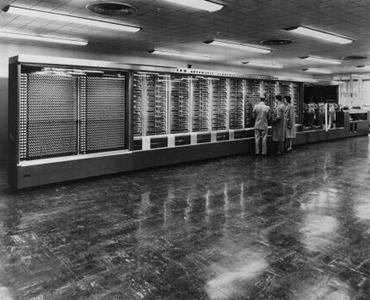
\includegraphics[width=.65\linewidth]{./Imagenes/ascc.jpg}}
		\caption{ASCC}
		\label{fig:ascc}
	\end{subfigure}%
	\begin{subfigure}{.5\textwidth}
		\centering
		\href{https://www-03.ibm.com/systems/z/hardware/z13.html}{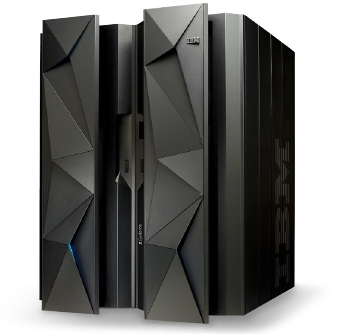
\includegraphics[width=.65\linewidth]{./Imagenes/z13.jpg}}
		\caption{Z13}
		\label{fig:z13}
	\end{subfigure}
\end{figure}



\subsection{Mainframes IBM z Systems}

\subsubsection{Blockchain}


\subsection{Watson}
En 2007 \href{https://www.research.ibm.com/}{IBM Research} se propuso el reto de crear un sistema para competir con los grandes campeones en el juego \href{https://www.jeopardy.com/}{Jeopardy!}. 
Este sistema, en adelante Watson, entraría dentro de la categoría QA (Question answering), que requiere avances en varias áreas de la ciencia de la computación y la inteligencia artificial. 
Algunas de estas áreas serían búsqueda y recuperación de información (IR), procesamiento de lenguaje natural (NLP), representación del conocimiento y razonamiento o el machine learning.

\begin{figure}[H]
	\centering
	\label{j-watson}
	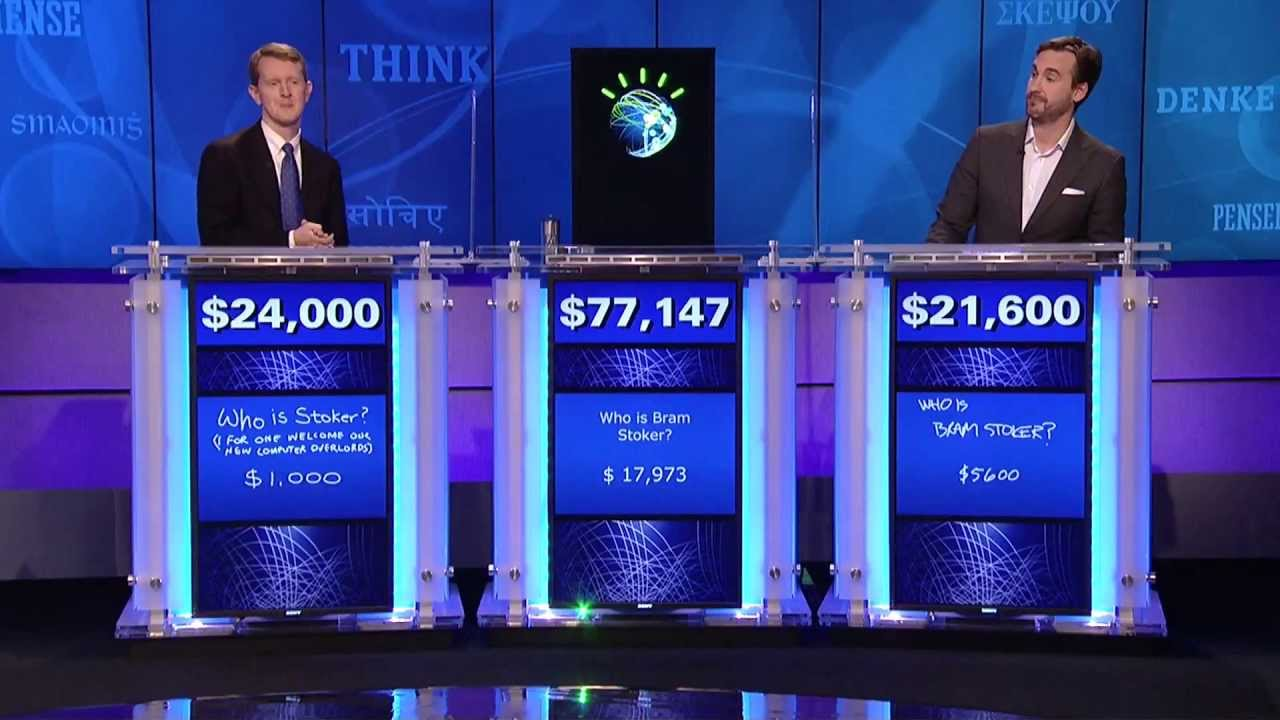
\includegraphics[width=0.7\textwidth]{./Imagenes/j-watson.jpg}
	\caption{Watson en Jeopardy!}
\end{figure}

\

La comunicación humana es imperfecta, está llena de ambigüedades, polisemia, ironías, la misma información puede darse de varias maneras y a veces la interpretación de una frase no solamente depende del contexto actual sino de conversaciones anteriores entre los interlocutores.
Además, dicha comunicación no está estructurada, como en un lenguaje de programación o una base de datos, donde los datos están bien definidos y la información es explícita.
A día de hoy la información no estructurada, como es el caso del lenguaje natural, crece más rápido que la estructurada, por ello es buena idea usar análisis profundos del lenguaje natural para hacer inferencia a partir de los datos de los que disponemos.
% this-is-watson: word-sense disambiguation [5, 6], latent semantic analysis [7], textual entailment [8], and coreference resolution [9]

\

Desde 2001 hasta 2006 se construyó la base para el reconocimiento de información no estructurada, UIMA (Unstructured
Information Management Architecture). % this-is-watson:[10]
UIMA proporciona una plataforma para integrar la información obtenida tras analizar textos, imágenes, etc.
Su objetivo es integrar varios programas llamados \textit{anotadores}, que asignan significado semántico a ciertas partes del texto o imagen.

% Watson was the system-level experiment that brought together hundreds of different cooperating algorithms, each of these algorithms alone performs relatively simple language processing tasks.
% In May 1997, IBM’s Deep Blue* computer beat Gary Kasparov (IBM Research beckoned for an encore)

Algunos desarrolladores habían participado anteriormente en Question answering dentro del proyecto PIQUANT \cite{piquant}. % this-is-watson [13, 14]
Este sistema tenía un conjunto estático de tipos de respuestas o clases de conceptos que se solicitaban en una pregunta.
El nuevo sistema no tendría conexión a Internet, y en unos tres segundos tendría que procesar la pregunta, buscar una respuesta y estimar la probabilidad de que sea correcta.
Tras analizar $2.000$ partidas de \textit{Jeopardy!} la media de los jugadores que ganaban era una precisión del $85-95\%$ de acierto sobre una media de $40-50\%$ de preguntas respondidas, o 
\textit{85\% Precision@40}


\subsubsection{Arquitectura}
En $2007$ se consiguió, usando PIQUANT, un rendimiento 16\% Precision@70 en las preguntas de \textit{Jeopardy!}.
Después se desarrollaron dos técnicas esenciales en el desarrollo de \textit{Watson}, DeepQA % this-is-watson: [4]
y AdaptWatson. % this-is-watson: [16,17]

\begin{figure}[H]
	\centering
	\label{tiw-deepqa}
	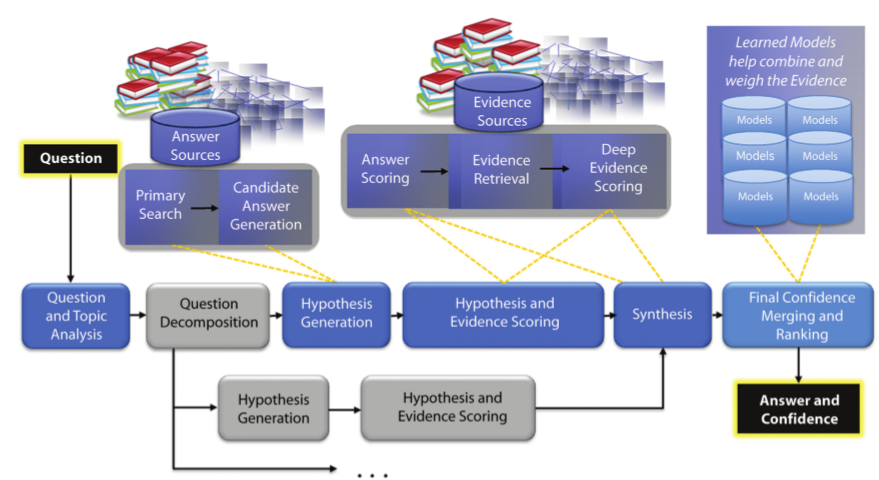
\includegraphics[width=0.8\textwidth]{./Imagenes/deepQA.png}
	\caption{Arquitectura DeepQA}
\end{figure}

\textbf{DeepQA} define varias etapas del análisis, cada una tiene diferentes implementaciones que se ejecutan en paralelo.  
Nunca se admite que se ha entendido perfectamente una pregunta, de forma que pueda verse directamente la respuesta en una base de datos.
Lo que se hace es buscar varias posibles preguntas candidatas, ponderar la probabilidad de que cada una sea la correcta, buscar varias posibles respuestas a cada pregunta y usar diferentes fuentes para ponderar la probabilidad de cada respuesta.
En dicho proceso se le da valor al hecho de que una respuesta concuerde con el tipo que se espera, por ejemplo un monumento histórico, una persona, etc.
También se tienen en cuenta fechas, geografía, la fiabilidad de las fuentes, etc.
Este análisis produce cientos de valores o características, cada uno indicando el grado de evidencia que se ha encontrado de cada tipo que refuerza una respuesta concreta.
Todas esas características deben ser combinados para obtener un único valor representando la probabilidad de que la respuesta sea correcta.
Para dar una ponderación a cada característica de DeepQA se entrenó con un modelo estadístico usando machine learning a partir de preguntas y respuestas
El resultado final es una lista de respuestas candidatas, cada una con un valor que nos indica si es buena respuesta o no, en función de la evidencia.

\

El rendimiento del sistema no era demasiado alto, hasta que consiguieron integrar diferentes técnicas algorítmicas usando una metodología llamada \textbf{AdaptWatson}.
Estos componentes actúan sobre la arquitectura de DeepQA con el objetivo de entender las preguntas, buscar respuestas candidatas y ponderar la confianza en dichas respuestas.
El equipo documentó más de $8.000$ experimentos independientes en el ciclo de vida de Watson, cada uno con $10-20GB$ de datos.
A partir de estos datos se buscaban fallos y sus posibles causas.
De esta forma se mejoró hasta un 85\% Precision@70.

\subsubsection{Entendiendo las preguntas}
Una pregunta tiene un tipo de respuesta potencial que llamaremos LAT (lexical answer type), además cada pregunta en \textit{Jeopardy!} tiene una categoría que ayudará a identificar el tema sobre el que se pregunta. % this-is-watson: question analysis algorithms [18]
Para entender las preguntas formuladas se usa un parser ESG (English Slot Grammar) % this-is-watson: [19]
y un generador PAS (predicate-argument structure). 

\begin{itemize}
	\item ESG identifica partes de la frase y roles sintácticos como el sujeto y relaciones entre las diferentes partes de la frase.
	\item El generador PAS es usado para producir una representación abstracta, que representa la interfaz con la parte analítica (otra capa de DeepQA de la resolución del problema.
\end{itemize}

En cuanto a las \textbf{respuestas y fuentes de evidencia} al principio se usaba añadieron enciclopedias y libros de referencia. Después se desarrolló un proceso semiautomático para hacer crecer el conocimiento de Watson, no se puede añadir contenido sin parar ya que afecta al rendimiento del sistema.
% this-is-watson: proceso para añadir conocimiento [20, 21]
Tras analizar el contenido que se añade se crea PRISMATIC, que extrae información y usa la estadística para deducir lo que es conocimiento base, esto ayudará en la parte de generación de respuestas candidatas y calcular sus probabilidades.
% this-is-watson: descubrir respuestas candidatas [22]

\

Cada una de las consultas usan información estructurada y no estructurada usando varios mecanismos de búsqueda complementarios.
Una pareja de consulta y respuesta representan una hipótesis.
% this-is-watson: generación de hipótesis [23]
Una métrica %(candidate binary recall)
que se usa para medir la bondad de una respuesta es el porcentaje de preguntas en las que dicha respuesta es generada como candidata. 
Esta medida ayuda a combinar los resultados, sobre todo cuando tenemos varias interpretaciones diferentes de lo que se está preguntando.
De esta forma se determina la probabilidad final de que una respuesta sea correcta para la pregunta inicial.
De las experiencias de los desarrolladores con el sistema PIQUANT sabían que no era una estrategia adecuada intentar anticipar todos los tipos de respuesta y crear algoritmos que busquen solamente instancias de dichas clases.
Esto es debido en parte a la complejidad de algunas preguntas, ya que todo el sistema se apoya en haber reconocido correctamente el tipo de respuesta necesaria, y que en el conocimiento del sistema dicha respuesta esté bien clasificada.
En la siguiente pregunta de la categoría \textit{decoración} el tipo de respuesta buscada es una \textit{dirección}:

\begin{center}
Si usted está de pie, es la dirección que debe buscar para ver el revestimiento.

\textbf{Respuesta}: Abajo
\end{center}



\

\begin{comment}
We employ
dynamic and flexible techniques for classifying candidate
answers, heavily relying on the context in the question.
For this, we developed a technique we called type coercion
[24]. Type coercion radically differs from earlier systems
(such as PIQUANT) that statically classify a possible answer
on the basis of a preexisting set of types

Watson uses an extensible ensemble
of techniques based on a wide variety of textual and
ontological resources, including PRISMATIC [21], YAGO
[25], and WordNet** [26].

In the next paper,
in the issue, BTyping Candidate Answers using Type
Coercion,[ Murdock et al. [27] discuss the type coercion
techniques developed for Watson that provide the dynamic
classification necessary for dealing with the huge variety of
contextual types used in Jeopardy!.

-- Collecting and scoring evidence
These algorithms are designed to produce a
confidence scoreVa number that indicates the degree to
which a piece of evidence supports or refutes the correctness
of a candidate answer.
Multiple evidence scorers can work
in parallel for each candidate answer and over different
forms of evidence

In BRelation Extraction and Scoring
in DeepQA,[ Wang et al. [29] present two approaches
to broad-domain relation extraction and scoring: one
based on manual pattern specification (rule based) and
the other relying on statistical methods for pattern elicitation,
which uses a novel transfer learning technique, relation
topics.

(approximately 30). Statistical approaches, on the other hand,
automatically learn how to extract semantic relations from
training data, which may be collected semiautomatically
and were trained to detect occurrences of a large number
of relations (approximately 7,000).

MOTHERS & SONS: Though only separated by one
year in real life, she played mother to son Colin Farrell
in BAlexander.[ (Answer: BAngelina Jolie[)
Relation: starring (she, BAlexander[)
Although structured resources tend to be too narrow and
brittle to directly and confidently answer questions, several
components in DeepQA do use structured data

--Puzzles, Final Jeopardy!, and other Special Questions

BEFORE & AFTER: The BJerry Maguire[ star who
automatically maintains your vehicle’s speed.
(Answer: BTom Cruise control[)

Special Questions are handled by a collection of algorithms
designed to first detect their occurrence

Missing links
Realizing and resolving implicit relationships and using
them to interpret language and to answer questions is
generally useful and appears in different forms in Jeopardy!
the ability to find what different
concepts have in common can help in many areas, including
relating symptoms to diseases

-- Breaking the question down
breaking a question down into logical subparts, so that the
subparts may be independently explored and the results
combined to produce the answer [36]

For example, in the clue below,
the system can independently find characters introduced
in 1894 and then words that come from Hindi for Bbear.[

FICTIONAL ANIMALS: The name of this character,
introduced in 1894, comes from the Hindi for Bbear.[
(Answer: BBaloo[)

--Merging evidence and combining confidence
For each of these answers, it may find
100 pieces of evidence in the form of paragraphs or facts
from databases. Each evidence-answer pair may be scored by
100 independent scorers.

Its job is to figure out the best way to combine
the confidence of many different scorers across different
pieces of evidence to produce a single probability for
each candidate answer.
This is done using a statistical
machine learning framework
normalization,
training with sparse training data, and merging related or
equivalent candidate answers.
Because machine learning is used
to weigh and combine scores, evidence scoring algorithms
can be easily introduced, revised, and reconfigured [37]

-- Massive parallelism, scale-out, and speed


- Planning for success required that we begin to consider latencyVthe
time it took to answer a question.
Watson would have to produce
its best answer and confidence estimation in an average of
about three seconds
At the end of 2008, DeepQA took about
two hours of CPU time to answer a Jeopardy! question,
running on a single 2.6-GHz processor with 16 GB of
memory.
UIMA-AS
allows any UIMA application to be deployed as a collection
of asynchronous processes that use standard messaging
infrastructure to communicate.
Each can be independently
scaled up, as needed, by deploying multiple instances of
the process on a larger number of machines.

First, each search query
could be independently executed. Subsequently, each
candidate answer could start a new independent thread of
processing, where each piece of evidence for each candidate
answer, could be independently scored

DeepQA was scaled out using UIMA-AS
using 2,880 processors to drive the QA latency down from
two hours to three seconds. [39]

-- Watson: An artificial Jeopardy! contestant
DeepQA refers to the architecture and implementation of a
system that takes a question and a category as input and
provides a ranked list of answers.
Each answer is associated
with probabilities that the answer is correct, based on
analyzed evidence.

1Decides which clues to select when Watson has control of
the board.
2Determines what to bet on Daily Doubles and on Final
3Determines a confidence threshold below which Watson
will not buzz in (even if it could) and above which
Watson will attempt to buzz in.


Watson into healthcare, we plan to move from taking
specific questions as input to analyzing entire problem
scenarios, represented, for example, by a patient’s electronic
medical record.
We imagine Watson 2.0 will support
mixed-initiative dialogue that extends over time as a problem
case is explored. This will allow the system to more
efficiently prune its search by gathering specific information
from the user.


\end{comment}


\section{Conclusiones}




%------------------------------------------------
\newpage
\bibliography{citas} %archivo citas.bib que contiene las entradas 
\bibliographystyle{plain} % hay varias formas de citar

\end{document}
